\section{参考代码中的当前方案}

\begin{itemize}
  \item \textbf{网络结构}\enspace H6 牵引训练在冻结的运动控制模型上增加速度修正 MLP。
  \item \textbf{网络输出}\enspace MLP 根据本体观测、历史特征和指令反馈，每帧直接输出前向、侧向和偏航速度修正的均值。训练将处理后的修正叠加到下一帧的原始指令。\ev{C2,C4}
  \item \textbf{训练参考}\enspace 平移参考修正在各轴的力分量越过阈值后立即饱和，偏航参考随拉力方向变化。奖励以速度修正误差为目标，未规定加速度或起步过渡曲线。\ev{C5,C6}
  \item \textbf{撤力响应}\enspace 撤力使参考修正归零，奖励鼓励 MLP 消除残余修正。原始指令也为零时，期望机器人停车。当前训练缺少显式停车约束。\ev{C5,C6,C7}
  \item \textbf{部署指令}\enspace H6 v2 优先采用摇杆或 Follow 外部指令。外部指令幅值连续 $0.4\,\mathrm{s}$ 低于 $0.1$ 后，切换到 C++ 后处理后的网络速度输出。\href{https://github.com/VitaDynamics/cerebrix/blob/57a05ee00d229da6fd6f10defcc51e947247d6c6/source/cerebrix/cerebrix/rl/traction/contracts/deployment_h6_v2/deployment_contract.json\#L57}{部署契约}
\end{itemize}

本节对应 \code{--teacher_aligned} 的基线配方与 \code{source_v1} 采样。训练入口为 \code{train_frozen_latent.py}。\ev{C1,C3}

\subsection{网络设计}

训练时的网络结构与反馈见图~\ref{fig:h6-network-feedback}。观测沿用式~\eqref{eq:proprio-observation} 和式~\eqref{eq:proprio-history}，
取 $H=6$，关节动作项使用上一控制步的平滑动作。仿真机身线速度和力标签用于奖励与 Critic。\ev{C2,C4,C6}

\begin{itemize}
  \item 前向、侧向、偏航修正的限幅依次为 $[-0.5,1.3]$、$[-0.5,0.5]$、$[-1.5,1.5]$。
  \item 平移与偏航绝对值的死区阈值分别为 $0.05\,\mathrm{m/s}$ 和 $0.05\,\mathrm{rad/s}$。
  \item 导出网络的 \code{action_cmd} 为修正均值，后处理在网络外执行。\ev{C2,C3,C5}
\end{itemize}

令缩放系数 $S=\operatorname{diag}(2,2,0.25)$，常规控制帧的指令输入满足\ev{C4}
\begin{equation}
 o_t[0{:}3]=S(\bm c^0_t+\bm\delta_{t-1}),\qquad
 \mathrm{cmd\_ori}_t=[S\bm c^0_t,\ S\bm\delta_{t-1}].
\label{eq:redundant}
\end{equation}

\begin{figure}[!htbp]
\centering
\begin{tikzpicture}[
  node distance=5mm,
  block/.style={draw=ink,fill=ink!4,rounded corners=2pt,
    text width=116mm,minimum height=11mm,align=center,
    inner sep=5pt,font=\small},
  input/.style={block,text width=43mm,minimum height=17mm},
  >={Stealth[length=2mm]},line width=0.7pt
]
\node[input] (obs) at (-52mm,0) {\textbf{最新帧观测}\\[2pt]
  $\bm o_t$（45 维）};
\node[input] (latent) at (0,0) {\textbf{CTS 历史特征}\\[2pt]
  $\bm z_t$（32 维）};
\node[input] (cmd) at (52mm,0) {\textbf{指令反馈}\\[2pt]
  \texttt{cmd\_ori}（6 维）};

\node[block,below=9mm of latent] (mlp) {\textbf{速度修正 MLP}\quad $83\to256\to128\to3$};
\node[block,below=of mlp] (process) {\textbf{修正处理与反馈}\\[2pt]
  修正均值 $\bm\mu_t$（3 维，前向、侧向、偏航）\\[2pt]
  训练时从均值对应的分布采样，经限幅与死区得到 $\bm\delta_t$\\[2pt]
  将 $\bm\delta_t$ 写入下一帧指令反馈与观测
  \quad $\bm c^{\rm obs}_{t+1}=S(\bm c^0_{t+1}+\bm\delta_t)$};
\node[block,below=of process] (base) {\textbf{冻结运动控制模型}\\[2pt]
  输入 $h_{t+1}$，输出 12 维关节动作 $\bm a_{t+1}$};

\draw[->] (obs.south) -- ++(0,-4mm) -| ([xshift=-35mm]mlp.north);
\draw[->] (latent.south) -- (mlp.north);
\draw[->] (cmd.south) -- ++(0,-4mm) -| ([xshift=35mm]mlp.north);
\draw[->] (mlp) -- (process);
\draw[->] (process) -- (base);
\end{tikzpicture}

\caption{H6 速度修正网络的输入、输出与下一帧反馈。}
\label{fig:h6-network-feedback}
\end{figure}

\clearpage
\subsection{训练环境与采样}

\noindent\textbf{外力采样与施加}\ev{C7}
\begin{itemize}
  \item \textbf{采样范围}\enspace 在机身坐标系均匀采样 $F_x,F_y\in[-50,50]\,\mathrm N$、$F_z\in[-10,10]\,\mathrm N$。
  \item \textbf{周期时序}\enspace 各环境每隔 $4\,\mathrm{s}$ 同步独立采样，前 $3.02\,\mathrm{s}$ 保留采样值，后 $0.98\,\mathrm{s}$ 清零。
  \item \textbf{施力方式}\enspace 保留采样值期间，每隔 $0.02\,\mathrm{s}$ 向机身 \code{base} 刚体质心施力一次，每次持续 $0.005\,\mathrm{s}$，附加力矩为零。
  \item \textbf{奖励用力}\enspace 计算参考速度修正时使用采样幅值。
\end{itemize}

\noindent\textbf{原始速度指令采样}\ev{C1,C3,C7}
\begin{itemize}
  \item \textbf{采样时机}\enspace \code{traction/commands.py} 在环境重置时及回合内每隔 $10\,\mathrm{s}$ 重采平移指令和目标航向。
  \item \textbf{平移指令}\enspace 前向速度由地形课程采样，侧向速度在 $[-0.3,0.3]\,\mathrm{m/s}$ 内均匀抽取。平移指令范数不超过 $0.1\,\mathrm{m/s}$ 时，两轴清零。
  \item \textbf{偏航指令}\enspace 通常每隔 $0.02\,\mathrm{s}$ 根据航向误差更新。
  \item \textbf{撤力后}\enspace 原始速度指令继续按上述时序更新。
\end{itemize}

\noindent\textbf{地形与动力学随机化}\ev{C1}
\begin{itemize}
  \item \textbf{地形}\enspace 沿用运动任务的粗糙地形课程。
  \item \textbf{动力学}\enspace 沿用地面摩擦、载荷与质心等随机化设置。
\end{itemize}

\subsection{由外力计算参考速度修正}

取机身坐标系下的水平力 $\bm F_{xy}=(F_x,F_y)$。平移参考速度修正通过下式计算
\begin{equation}
 g(F;l,u)=\begin{cases}
 0,& |F|\le\alpha,\\
 \clip\left(\dfrac{F+\alpha\sgn(F)}{\beta},l,u\right),&|F|>\alpha,
 \end{cases}
 \qquad
 \begin{aligned}
 \delta_{x,\rm ref}&=g(F_x;-0.5,1.2),\\
 \delta_{y,\rm ref}&=g(F_y;-0.5,0.5).
 \end{aligned}
\label{eq:force-map}
\end{equation}
基线取 $\alpha=17.5\,\mathrm N$、$\beta=20\,\mathrm{N\,s/m}$。代码中的 $(F/\beta)(1+\alpha/|F|)$ 与式~\eqref{eq:force-map} 的非零分支等价。H6 \code{teacher_aligned} 基线将前向参考速度修正上限设为 $1.2\,\mathrm{m/s}$，原始配方的上限为 $1.0\,\mathrm{m/s}$。\ev{C3,C5}

偏航参考速度修正由力的方向角 $\theta=\operatorname{atan2}(F_y,F_x)$ 决定
\begin{equation}
 \delta_{\omega,\rm ref}=\begin{cases}
 \clip\left(\dfrac{\theta+0.6\sgn(\theta)}{2},-0.8,0.8\right),
 &\|\bm F_{xy}\|>17.5\,\mathrm N\ \text{且}\ |\theta|>0.6\,\mathrm{rad},\\
 0,&\text{其余情况}.
 \end{cases}
\end{equation}
参考速度修正按当前力标签逐步计算，力标签清零时参考速度修正随即归零。\ev{C3,C5,C7}

图~\ref{fig:force-reference-map} 直接调用 \code{source_force_to_velocity} 计算，并与原始奖励映射函数 \code{_get_force_to_vel} 逐点核对。平移分量越过 $17.5\,\mathrm N$ 阈值后立即饱和；偏航分量同时受水平力幅值和方向角控制。\ev{C3,C5}

\noindent\begin{minipage}{\linewidth}
\captionsetup{hypcap=false}
\centering
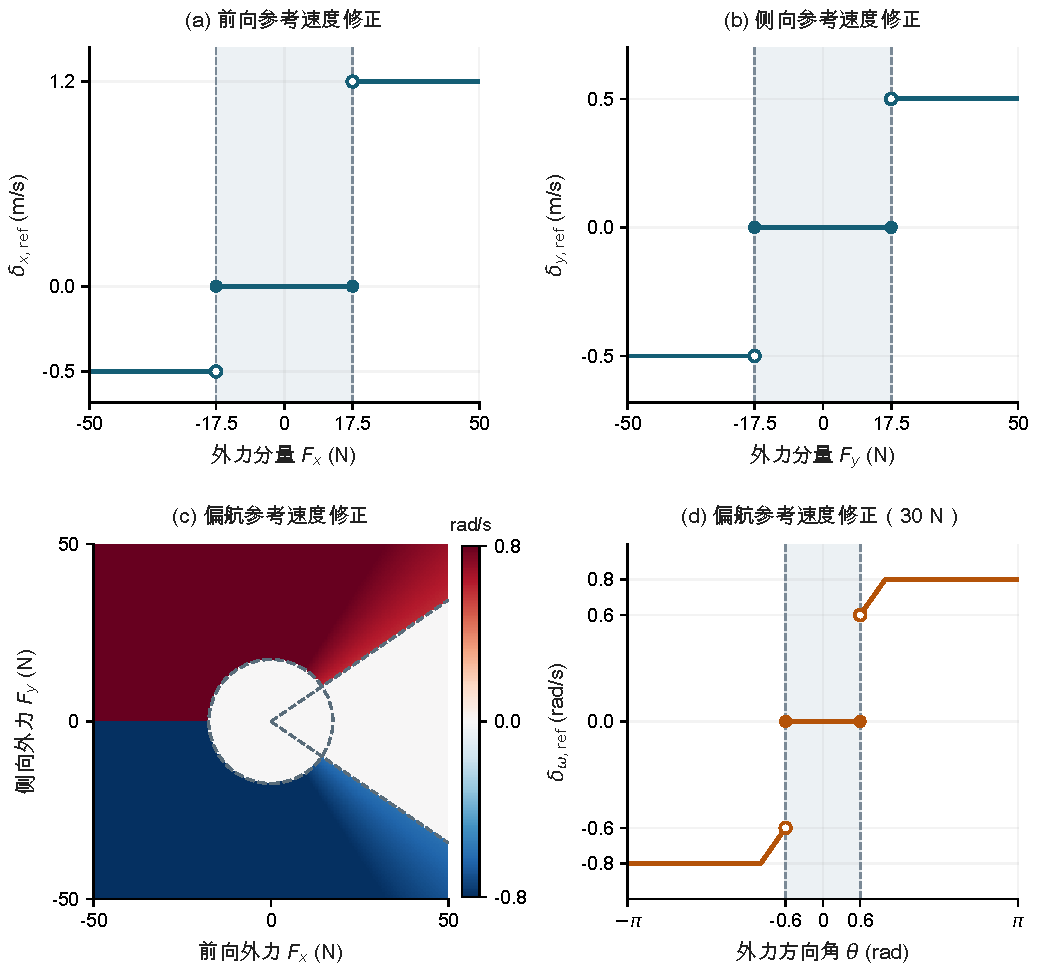
\includegraphics[width=0.84\linewidth]{figures/reference_map.pdf}
\captionof{figure}{外力与参考速度修正的关系。参数采用 H6 基线。子图 (a)、(b) 为前向、侧向映射；(c) 为偏航参考速度修正在水平力平面中的分布；(d) 为水平拉力大小固定为 $30\,\mathrm N$ 时，偏航参考速度修正随拉力方向的变化。实心点表示阈值处取值，空心点表示非零分支的极限，阴影表示死区。}
\label{fig:force-reference-map}
\end{minipage}\par

\subsection{奖励设计}

\noindent\textbf{牵引任务}\quad
\code{compliance} 比较本帧处理后的修正 $\bm\delta_t$ 与当前力标签生成的参考速度修正 $\bm\delta_{\rm ref,t}$。\ev{C6}
\begin{equation}
 r_{\rm comp,t}=-\|\bm\delta_{xy,t}-\bm\delta_{xy,\rm ref,t}\|^2
 -0.05(\delta_{\omega,t}-\delta_{\omega,\rm ref,t})^2.
\label{eq:comp}
\end{equation}

\noindent\textbf{运动跟踪}\quad
当前实现沿用底层运动跟踪奖励。跟踪目标为 $\bm c_{\rm trk,t}=\bm c^{0,\rm rew}_t+\bm\delta_{t-1}$，其中 $\bm c^{0,\rm rew}_t$ 是物理步结束后更新的原始指令，$\bm v_{xy,t}$ 和 $\omega_{z,t}$ 是此时的仿真机身速度。\ev{C6,C7}
\begin{align}
 r_{v,t}&=\exp\left(-\frac{\|\bm c_{\rm trk,xy,t}-\bm v_{xy,t}\|^2}{0.25}\right),&
 r_{\omega,t}&=\exp\left(-\frac{(c_{\rm trk,\omega,t}-\omega_{z,t})^2}{0.25}\right).
\end{align}
上述三项权重依次为 $5$、$1$、$0.5$，与其他奖励加权求和后乘控制步长。运动跟踪通过 PPO 回报影响牵引 MLP 学到的修正。物理步结束后更新力标签并计算奖励，新标签对应下一控制步排队施加的力。\ev{C6,C7,C8}

\noindent\textbf{稳定性与 PPO}\quad
其余奖励包含近零指令下的站姿、姿态、碰撞和关节动作平滑等。关节位置、力矩和速度限位作为三路约束代价。PPO 更新修正 MLP、采样标准差及奖励和代价 Critic，底座在牵引训练期间冻结。\ev{C6,C8}\cite{schulman2017}
